\documentclass[final,10pt]{beamer}  % This file used the rawExample.tex file as a starting point. I then changed
  \mode<presentation>          % the style sheet and looked at Kristin's poster to go from there
  {
% you can chose your theme here:
\usetheme{Icy}
% further beamerposter themes are available at
% http://www-i6.informatik.rwth-aachen.de/~dreuw/latexbeamerposter.php
}
\usepackage{type1cm}
\usepackage{calc}
\usepackage{times}
\usepackage{amsmath,amsthm, amssymb, latexsym}
%\boldmath
\usepackage[english]{babel}
\usepackage[latin1]{inputenc}
\usepackage[orientation=portrait,scale=1.3,debug]{beamerposter}
\setlength{\paperwidth}{46in}
\setlength{\paperheight}{34in}


%\definecolor{orange}{HTML}{F66733}


\usepackage{array,booktabs,tabularx,multirow}
\newcolumntype{Z}{>{\centering\arraybackslash}X} % centered tabularx columns
\newcommand{\pphantom}{\textcolor{ta3aluminium}} % phantom introduces a vertical space in p formatted table columns??!!


\newcommand{\B}{\boldsymbol}  % To make bold easier

\usepackage[center]{subfigure}
\usepackage{caption}

\usefonttheme{professionalfonts}

\graphicspath{{C:/Users/carle/Desktop/Poster4Carl}}


\title[]{\large Nonparametric Functional Calibration of Computer Models}
\author[Brown, Atamturktur]{\small {\em D. Andrew Brown} \inst{a} \and  Sez Atamturktur \inst{b} }
\institute[Clemson University]{\tiny \inst{a} Department of Mathematical Sciences, Clemson University, Clemson, SC, USA 29634\and
                                \inst{b} Glenn Department of Civil Engineering, Clemson University, Clemson, SC, USA 29634}
%\newcommand{\footlinetext}{Lehrstuhl f\"ur Informatik 6 - Computer Science Department - RWTH Aachen University - Aachen, Germany \par Mail: \texttt{<surname>@cs.rwth-aachen.de} \hfill WWW: \texttt{http://www-i6.informatik.rwth-aachen.de}\vskip1ex}
\date{}

\newlength{\columnheight}
\setlength{\columnheight}{72cm}


\def\insertframetitle{}
\def\footleft{}
\def\footright{}


\setbeamercolor{block title}{fg=green,bg=white} % Colors of the block titles
\setbeamercolor{block body}{fg=black,bg=white} % Colors of the body of blocks
\setbeamercolor{block alerted title}{fg=white,bg=dblue!70} % Colors of the highlighted block titles
\setbeamercolor{block alerted body}{fg=black,bg=dblue!10} % Colors of the body of highlighted blocks

\begin{document}
\begin{frame}{}\
    \begin{columns}[t]
    \begin{column}{.33\textwidth}
        \begin{beamercolorbox}[center, wd=1.175\textwidth]{postercolumn}
        \begin{minipage}[T]{\textwidth}
        \parbox[t][\columnheight]{\textwidth}{ % must be some better way to set the the height, width and textwidth simultaneously
        % Since all columns are the same length, it is all nice and tidy.  You have to get the height empirically
        % ---------------------------------------------------------%
        % fill each column with content
        \begin{block}{Computer Experiments}
            {\small
          \begin{itemize}\itemsep2ex
              \item Many phenomena studied in engineering and science are driven by complex processes.\\

              \item Physical experiments may be difficult to conduct because of economic, technical, or ethical limitations.\\

              \item
              Today, the use of computer simulations as proxies for resource-intensive physical data is common.

              \item Examples:
                    \begin{itemize}
                        \item
                        Large-scale climate models

                        \item
                        Plastic deformation of materials under extreme conditions

                        \item
                        Performance of experimental prosthetic devices
                    \end{itemize}

          \end{itemize}
          }
          \hfill {\tiny Sacks et al. (1989), Santner et al. (2003)}
        \end{block}
        \vfill

         \begin{block}{Computer Model Calibration}
            {\small
            \begin{itemize}\itemsep2ex
              \item
              Utility of any computer model depends on the model's fidelity to reality

              \item
              \textcolor{orange}{Model Calibration}: Determine appropriate values of parameters in the computer code so that the output closely approximates physical observations


                \item
                Experimental design (control) settings: $\B{x}_i \in [0, 1]^{d_x}, ~i= 1,\ldots, N, ~d_x \geq 1$

                \item
                True parameter values under which the computer model agrees with reality: $\boldsymbol{\theta}$

                \item
                Representation:
                \[
                    \underbrace{y(\B{x}_i)}_{\text{field data}} = \underbrace{\eta(\B{x}_i, \boldsymbol{\theta})}_{\text{computer output}} + \underbrace{\epsilon_i}_{\text{Gaussian error}}
                \]

                \item
                The \textcolor{orange}{Bayesian approach} is to assign $\boldsymbol{\theta}$ a prior and base predictions on the posterior predictive distribution of $y_i$

                \item
                Priors elicited from subject matter experts are often necessary to account for weakly identifiable parameters

            \end{itemize}
            }
            \hfill {\tiny Kennedy and O'Hagan (2001), Bayarri et al. (2007), Higdon et al. (2008)}
        \end{block}
        \vfill

        \begin{block}{Functional Calibration}
        {\small
          \begin{itemize}\itemsep2ex
              \item
              Standard practice is to assume $\boldsymbol{\theta}$ is fixed throughout the domain of control inputs

              \item
              Often in application, \textcolor{orange}{the best settings for the calibration parameters may change with different control inputs}

              \item
              Goal: Model calibration parameters as smooth nonparametric functions of the control inputs, while accounting for expert-elicited prior constraints

          \end{itemize}
          }
          \hfill {\tiny Fugate et al. (2006), Atamturktur et al. (2015), Pourhabib et al. (2015), Plumlee et al. (2016)}
          %\vfill
        \end{block}
        }
        \end{minipage}
        \end{beamercolorbox}
    \end{column}

    \begin{column}{.33\textwidth}
    \begin{beamercolorbox}[center,wd=1.325\textwidth]{postercolumn}
    \begin{minipage}[T]{\textwidth}
    \parbox[t][\columnheight]{\textwidth}{ % must be some better way to set the the height, width and textwidth simultaneously
    % Since all columns are the same length, it is all nice and tidy.  You have to get the height empirically
    % ---------------------------------------------------------%
    % fill each column with content

        \begin{block}{Contribution: State-Aware Calibration}
            {\small
            \begin{itemize}\itemsep2ex
            \item
            Partition parameters into functional ($\B{\theta}_1(\B{x})$) and constant ($\B{\theta}_2$) parameters and assume independence {\em a priori}:
            \[
                \pi(\B{\theta}(\B{x})) = \pi_1(\B{\theta}_1(\B{x}))\pi_2(\B{\theta}_2)
            \]

            \item
            \textcolor{orange}{Nonparametric Gaussian process model for $\B{\theta}(\cdot)$}

            \item
            Scale $\B{\theta}$ to lie in the unit hypercube to honor expert-elicited bounds
            \begin{itemize}
                \item
                Use an appropriate link function to avoid boundary issues
            \end{itemize}
            \end{itemize}

            {\small
            \begin{eqnarray*}  % 4 in the correlation function: |x - x'| = |1/2| => r(x,x') = \rho
                g(\theta_{1i}(\cdot)) &\stackrel{\text{indep.}}{\sim}& \mathcal{GP}(\mu_{\theta,i}, ~\lambda_{\theta,i}^{-1}R_i(\cdot, \cdot))\\
                R_i(\mathbf{x}, \mathbf{x}^{\prime}) &=& \exp\left\{-4\sum_{k=1}^{d_x}\gamma_{\theta,i,k}|x_k - x_k^{\prime}|^2\right\}
            \end{eqnarray*}
            }

            where $g:(0,1) \rightarrow \mathbb{R}$ is one-to-one and differentiable, $\lambda_{\theta,i}$ are the unknown precisions, and $\gamma_{\theta,i,k}$ controls the smoothness of $\theta_{1i}(\cdot)$ along the $k^{\text{th}}$ direction
          %\end{itemize}
          }
          %\vfill

          \hfill {\tiny McCullagh and Nelder (1989), Rasumssen and Williams (2006)}
        \end{block}
        \vfill
%        }
%        \end{minipage}
%        \end{beamercolorbox}
%    \end{column}




%    \begin{column}{.33\textwidth}
%        \begin{beamercolorbox}[center,wd=\textwidth]{postercolumn}
%        \begin{minipage}[T]{.95\textwidth}
%        \parbox[t][\columnheight]{\textwidth}{ % must be some better way to set the the height, width and textwidth simultaneously
%        % Since all columns are the same length, it is all nice and tidy.  You have to get the height empirically
%        % ---------------------------------------------------------%
%        % fill each column with content
        \begin{block}{Ex: Two-Parameter Model with Scalar Control}
            {\small
            Proposed model:
            \begin{equation*}
            \begin{aligned}
                \mathbf{y} \mid \boldsymbol{\theta}^{(\mathbf{x})}, ~\lambda_y &\sim N_N(\boldsymbol{\eta}(\boldsymbol{\theta}^{(\mathbf{x})}), ~\lambda_y^{-1}\mathbf{I})\\
                \lambda_y &\sim \text{Ga}(a_y, ~b_y), ~~a_y, b_y > 0\\
                g(\theta_1(\cdot)) \mid \lambda_{\theta}, ~\rho_{\theta} &\sim \mathcal{GP}(\mu_{\theta}, ~\lambda_{\theta}^{-1}R_{\rho_{\theta}}(\cdot, \cdot)), ~~-\infty < \mu_{\theta} < \infty\\
                \theta_2 &\sim \text{Unif}(0, 1)\\
                \lambda_{\theta} &\sim \text{Ga}(a_{\theta}, ~b_{\theta}), ~~a_{\theta}, b_{\theta} > 0\\
                \rho_{\theta} &\sim \text{Beta}(1, ~b_{\theta}), ~~b_{\theta} > 0,
            \end{aligned}
        \end{equation*}

        where $\boldsymbol{\eta}(\boldsymbol{\theta}^{(\mathbf{x})}) = (\eta(x_1, \theta_1(x_1), \theta_2), \ldots,$ $\eta(x_N, \theta_1(x_N), \theta_2))^T$, $\boldsymbol{\theta}_1^{(\mathbf{x})} = (\theta_1(x_1), \ldots, \theta_1(x_N))^T$, and $R_{\rho_{\theta}}(x, ~x^{\prime}) = \rho_{\theta}^{4(x - x^{\prime})^2}$\\

        \begin{itemize}\itemsep2ex
            \item
            Enforce smoothness through choice of $b_{\theta}$
            \begin{itemize}
                \item
                E.g., $b_{\theta}= 0.1$ or $b_{\theta} = 0.2$
            \end{itemize}

            \item
            Standardized data $\Rightarrow$ concentrate $\lambda_y$ near one
        \end{itemize}

        }
            \hfill {\tiny Atamturktur and {\bf {\tiny B}} (2015), {\bf {\tiny B}} and Atamturktur (2016)}
        \end{block}
        \vfill


        \begin{block}{Implementation (MCMC)}
            {\small
            \begin{itemize}\itemsep2ex
            \item
            Eliminate boundary constraints with $\xi = \log(-\log(\theta_2))$ and $\nu = \log(-\log(\rho_{\theta}))$

            \item
            Metropolis proposal $(g(\theta_1^{\dagger}(x_1)), \ldots, g(\theta_1^{\dagger}(x_N)))^T \sim MVN$ with correlation matrix dependent upon the current value of $\rho_{\theta}$


            \item
            Observed design points close together $\Rightarrow$ \textcolor{orange}{correlation matrix is numerically unstable}
            \begin{itemize}
                \item
                Add a `nugget': $\mathbf{R}_{\nu, \delta} := \mathbf{R}_{\nu} + \delta\mathbf{I}$

            \end{itemize}

            \end{itemize}
          %\vfill
          \hfill {\tiny Tierney (1994), Neal (1998, 2011), Qian and Wu (2008), Ranjan et al. (2011)}
        }
        \end{block}
        \vfill
        } % end parbox
        \end{minipage}
        \end{beamercolorbox}
    \end{column}

    \begin{column}{.33\textwidth}
    \begin{beamercolorbox}[center,wd=1.475\textwidth]{postercolumn}
    \begin{minipage}[T]{\textwidth}
    \parbox[t][\columnheight]{\textwidth}{ % must be some better way to set the the height, width and textwidth simultaneously
    % Since all columns are the same length, it is all nice and tidy.  You have to get the height empirically
    % ---------------------------------------------------------%
    % fill each column with content

        \begin{block}{Simulation Study}
        {\small
            \begin{itemize}\itemsep2ex

                \item
                Truth: $y(x_i) = \underbrace{c_1(x_i)}_{= 2\sqrt{x_i}} + \underbrace{c_2}_{= 2.5}x_i^2 + \varepsilon_i, ~~\varepsilon_i \stackrel{\text{iid}}{\sim}N(0, ~0.05^2)$

                \item
                Computer model: $\eta(x, t_1, t_2) = t_1 + t_2 x^2$

                \item
                Field data generated at $\mathbf{x} = (0.00, 0.05, 0.10, \ldots, 0.90, 0.95)^T$; responses $\mathbf{y}^{\ast} = (y(0.45), \ldots, y(0.65))^T$ held out for validation

            \end{itemize}
%        }
%        \end{block}
%        \vfill
%
%        \begin{block}{Results }
%        {\small
            \begin{figure}[tb]
            \centering
            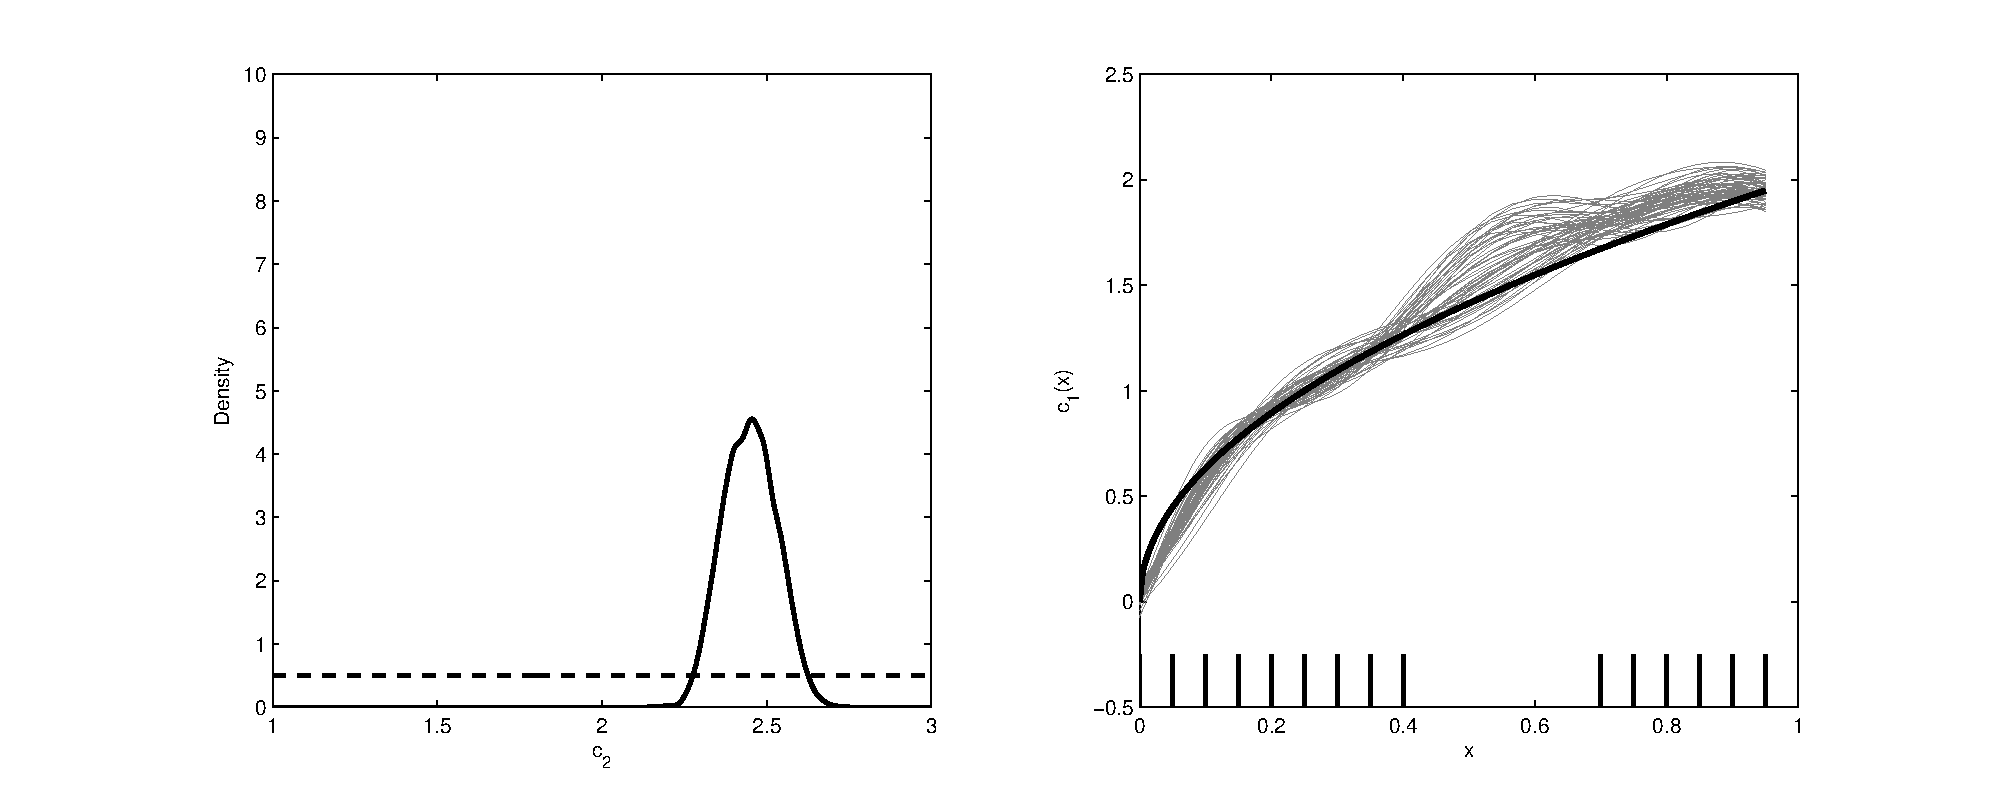
\includegraphics[scale= 0.5, clip= TRUE, trim= 0.5in 0pt 0in 0in]{strongTauPostPlots_2_Logit.eps}  % <- Laptop formatting
            %\includegraphics[scale= 0.575, trim= 1.4in -3.5in -1.75in 3.5in]{strongTauPostPlots_2.eps}  % <- Office PC formatting
            %\begin{singlespace}
            \caption{{\small Posteriors of $c_1(\cdot)$ and $c_2$ under the logit link with constraints on the boundary values of $c_1(\cdot)$. The dashed and solid curves in the left panel are the prior and posterior densities of $c_2$, respectively. The thick line in the right panel is the true function $c_1(\cdot)$.}}%\label{fig:strongTauPlots}
            %\end{singlespace}
        \end{figure}
        %\vfill

        \begin{figure}[tb]
            \centering
            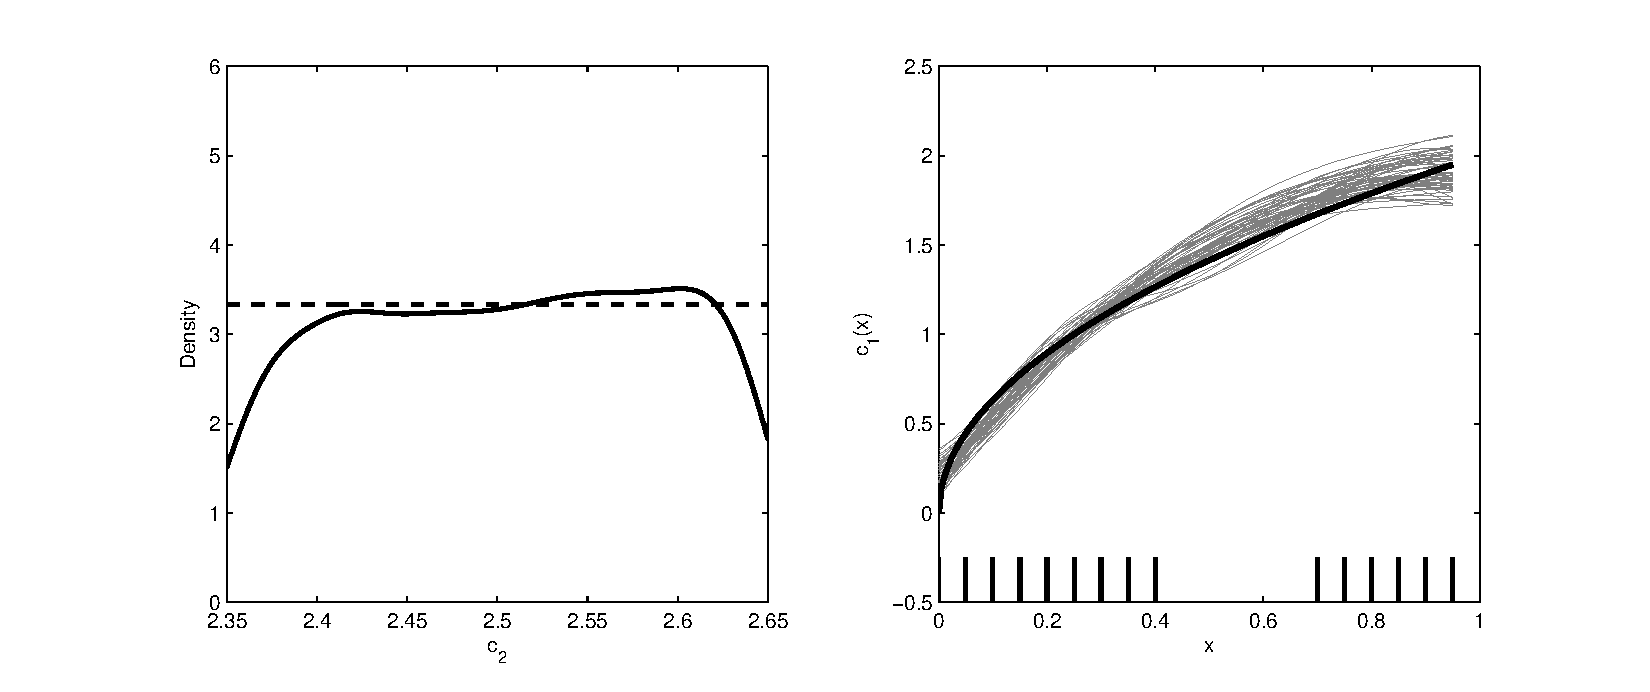
\includegraphics[scale= 0.6, clip= TRUE, trim= 0in 0pt 0in 0in]{strongN0PostPlots_2_Logit.eps}  % <- Laptop formatting
            % \includegraphics[scale= 0.6, trim= .5in -3.75in -1.75in 3in]{strongN0PostPlots_2.eps}  % <- Office PC formatting
            %\begin{singlespace}
            \caption{{\small Posteriors of $c_1(\cdot)$ and $c_2$ with logit link and tight prior bounds on $c_2$. The dashed and solid curves in the left panel are the prior and posterior densities of $c_2$, respectively. }}%\label{fig:strongN0Plots}
            %\end{singlespace}
        \end{figure}

       % \vfill


        \begin{figure}[tb]
            \centering
            \includegraphics[scale= 0.6, clip= TRUE, trim= 0in 0pt 0in 0in]{constTauPostPlots_2.eps}  % <- Laptop formatting
            % \includegraphics[scale= 0.6, trim= .25in -3.5in -1in 3in]{constTauPostPlots_2.eps}  % <- Office PC formatting
            %\begin{singlespace}
            \caption{Smoothed approximate posterior distributions of $c_2$ and $c_1$ when replacing the GP prior on $\theta_1(\cdot)$ with $\theta_1 \sim \text{Uniform}$.}%\label{fig:constTauPlots}
            %\end{singlespace}
        \end{figure}


        \begin{figure}[tb]
            \centering
            \includegraphics[scale= 0.5, clip= FALSE, trim= 0.25in 0in 0in 0in]{origDataHoldout_2_Logit_Rev1.eps}  % <- Laptop formatting
            %\includegraphics[scale= 0.5, trim= 2in -3.25in -2in 2.5in]{origDataHoldout_2_Improved.eps}  % <- Office PC formatting
            %\begin{singlespace}
            \caption{\textcolor{orange}{Strong disagreement between calibrated code and field data when assuming constant parameters}}%\label{fig:origData}
            %\end{singlespace}
        \end{figure}
        }
       % \vfill
        \end{block}
        \vfill

        \begin{block}{Summary}
            {\small
            \begin{itemize}\itemsep2ex
            \item
            Proposed model adequately captures functional behavior

            \item
            \textcolor{orange}{Erroneously assuming constant parameters can be misleading}

            \item
            Similar results from logit, probit, and identity link functions

            \end{itemize}
          %\vfill
        }
        \end{block}

%        } %end parbox
%        \end{minipage}
%        \end{beamercolorbox}
%    \end{column}





%    \begin{column}{.33\textwidth}
%        \begin{beamercolorbox}[center,wd=\textwidth]{postercolumn}
%        \begin{minipage}[T]{.95\textwidth}
%        \parbox[t][\columnheight]{\textwidth}{ % must be some better way to set the the height, width and textwidth simultaneously
%        % Since all columns are the same length, it is all nice and tidy.  You have to get the height empirically
%        % ---------------------------------------------------------%
%        % fill each column with content
        }%End parbox
        \end{minipage}
        \end{beamercolorbox}
    \end{column}

    \begin{column}{.33\textwidth}
        \begin{beamercolorbox}[center,wd=1.625\textwidth]{postercolumn}
        \begin{minipage}[T]{\textwidth}
        \parbox[t][\columnheight]{\textwidth}{ % must be some better way to set the the height, width and textwidth simultaneously
        % Since all columns are the same length, it is all nice and tidy.  You have to get the height empirically
        % ---------------------------------------------------------%
        % fill each column with content
        \begin{block}{Application: VPSC Plastic Deformation}
            {\small
            \begin{itemize}\itemsep2ex
                \item
                Model for plastic deformation of viscoplastic self-consistent (VPSC) materials

                \item
                Experiments with 5182 aluminum (to which VPSC is applicable) applied strain to each specimen up to 0.6, after which the stress is recorded.

                \item
                VPSC computer code:
                \[
                    \underbrace{y}_{\text{stress}} = \eta(\underbrace{x}_{\text{temperature}}, \underbrace{\theta_1(x)}_{\text{critical resolved shear stress}}, \underbrace{\theta_2}_{\text{inverse rate sensitivity}}) + \epsilon
                \]
            \end{itemize}

                \hfill {\tiny Lebensohn and Tom\'{e} (1993), Stout et al. (1998), Atamturktur et al. (2015)}

            }
        \end{block}
        \vfill


        \begin{block}{Results}
        {\small
        \begin{figure}[tb]
            \centering
            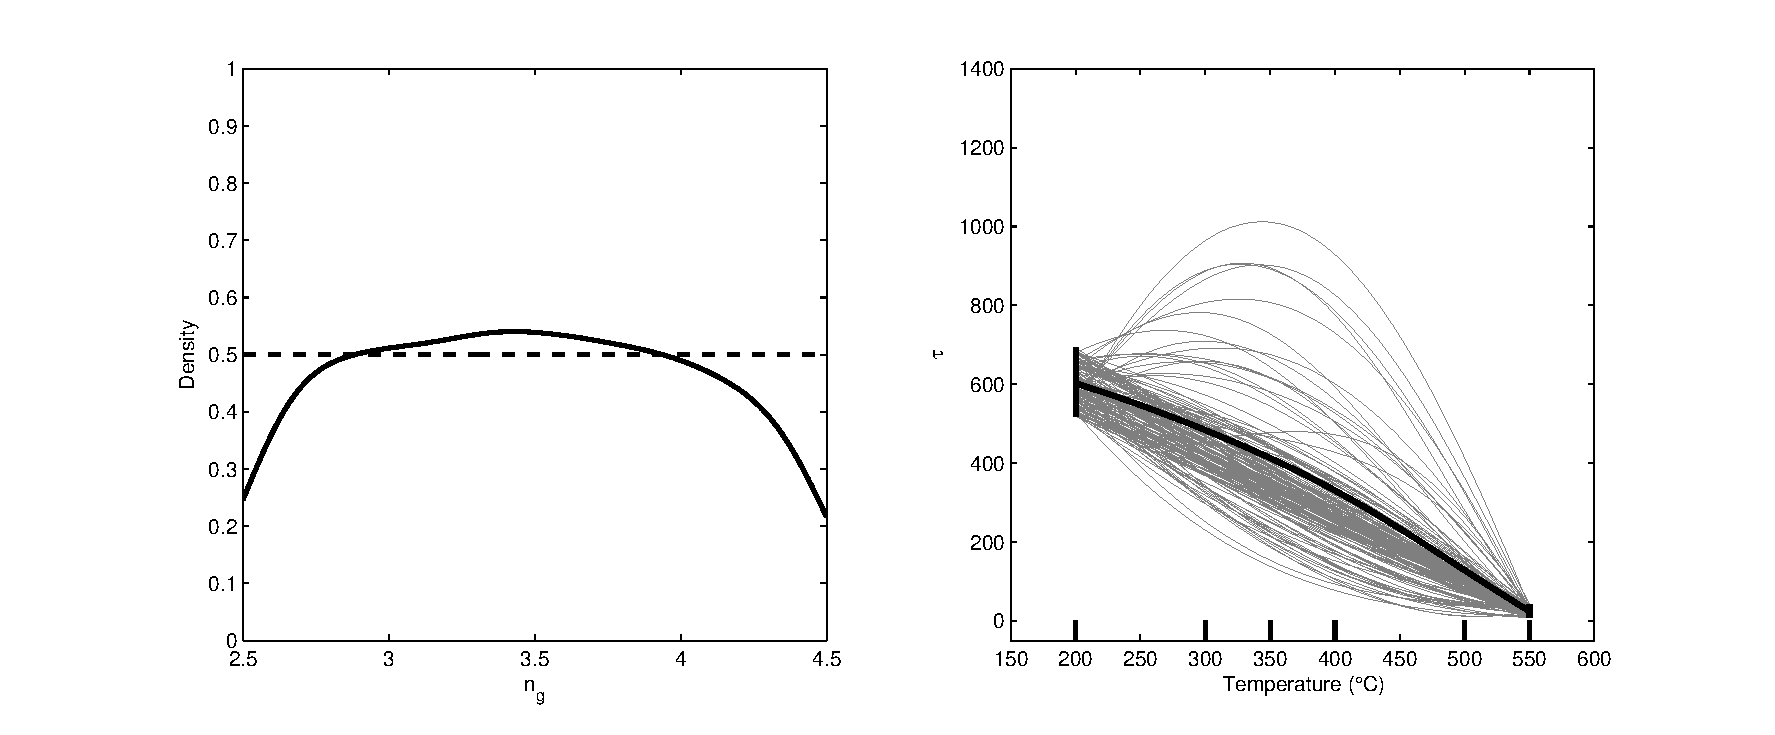
\includegraphics[scale= 0.55, clip= TRUE, trim= 0in 0pt 0in 0in]{VPSC_G_PostPlots_CleanedUp.eps}  % <- Laptop formatting
            % 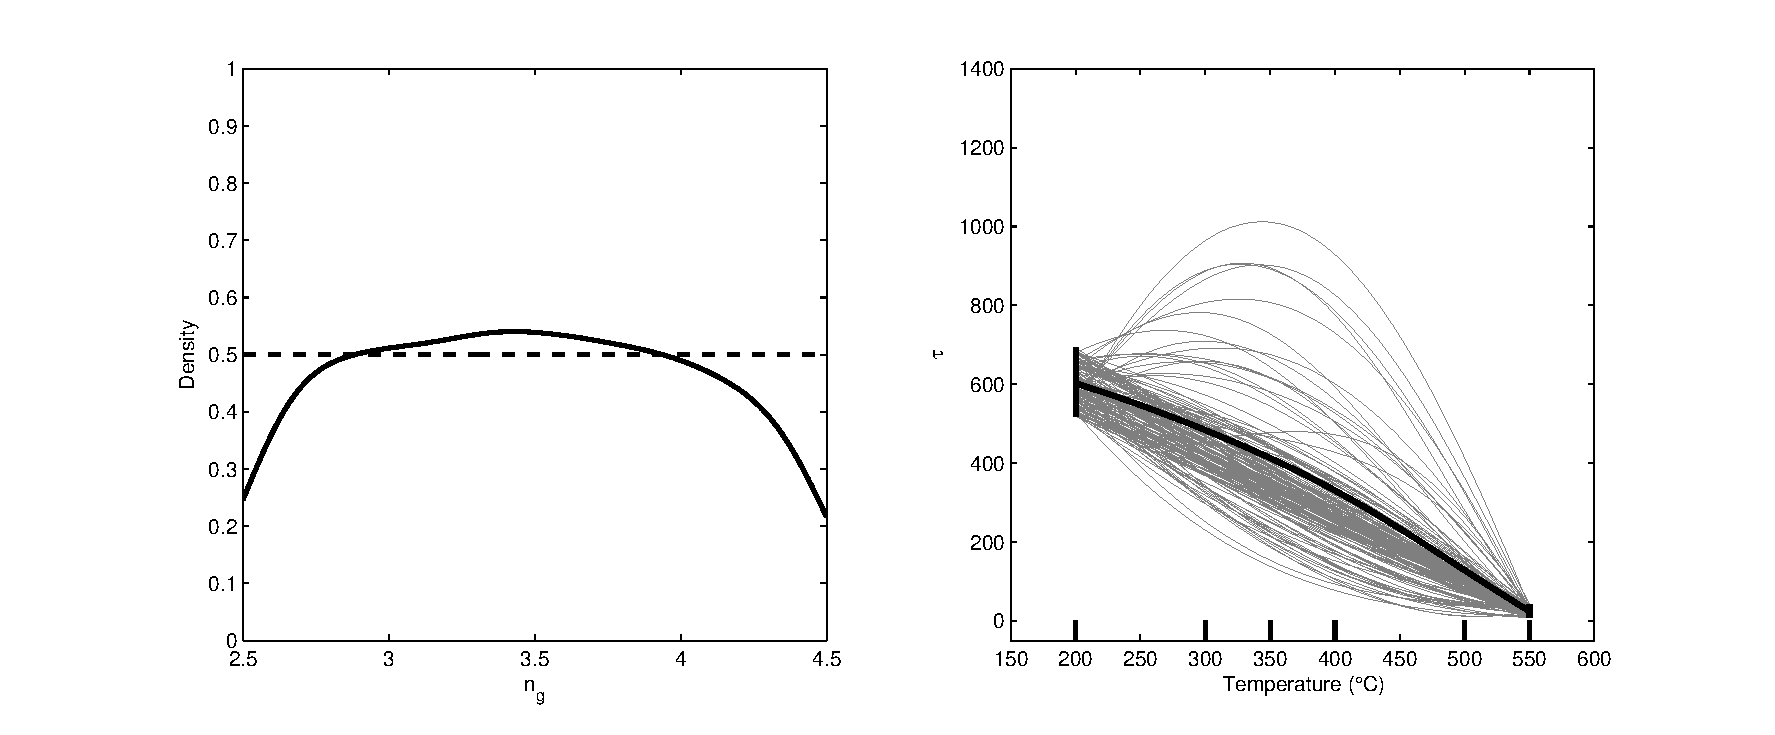
\includegraphics[scale= 0.55, trim= 1.75in -3.25in -1.75in 2.5in]{VPSC_G_PostPlots_CleanedUp.eps}  % <- Office PC formatting
            %\begin{singlespace}
            \caption{Smoothed prior and posterior histogram for inverse rate sensitivity (left panel) and sample paths drawn from the posterior of shear stress (right panel). The dark curve in the center is the pointwise mean of the sample paths; the vertical lines on the boundaries indicate the prior constraints imposed on the curves.}
            %\end{singlespace}
        \end{figure}

        \begin{itemize}\itemsep2ex
            \item
            Results agree with previous empirical work

            \item
            Model adequacy checks indicate modeling assumptions are consistent with experimental data
        \end{itemize}

        }
        \end{block}
        \vfill

         \begin{block}{Conclusions}
            {\small
          \begin{itemize}\itemsep2ex
                \item
                Proposed approach \textcolor{orange}{incorporates prior information and fully accounts for uncertainty}.

                \item
                Assuming constant parameters may be misleading. \textcolor{orange}{A researcher may include an empirical discrepancy term when functional calibration is needed}.

                \item
                When to invoke state-aware calibration?
                \begin{enumerate}
                    \item
                    Begin with conventional (all constant) calibration

                    \item
                    Systematic model bias $\Rightarrow$ consider functional relationships

                    \item
                    Sensitivity analysis to identify likely functional parameters

                    \item
                    Compare nonparametric and parametric models
                \end{enumerate}

            \end{itemize}
          }
          %\vfill
        \end{block}
        \vfill

        \begin{block}{Reference}
            {\small

            Brown, D. A. and Atamturktur, S. (2018), ``Nonparametric functional calibration of computer models," {\em Statistica Sinica}, to appear. \url{doi:10.5705/ss.202015.0344}

            }
        \end{block}


        }%End parbox
        \end{minipage}
        \end{beamercolorbox}
    \end{column}
 %
%      \begin{column}{.3\textwidth}
%        \begin{block}{Introduction}
%          \begin{itemize}
%          \item some items and $\alpha=\gamma, \sum_{i}$
%          \item some items
%          \item some items
%          \item some items
%          \end{itemize}
%          $$\alpha=\gamma, \sum_{i}$$
%        \end{block}
%
%        \begin{block}{Introduction}
%          \begin{itemize}
%          \item some items
%          \item some items
%          \item some items
%          \item some items
%          \end{itemize}
%        \end{block}
%
%        \begin{block}{Introduction}
%          \begin{itemize}
%          \item some items and $\alpha=\gamma, \sum_{i}$
%          \item some items
%          \item some items
%          \item some items
%          \end{itemize}
%          $$\alpha=\gamma, \sum_{i}$$
%        \end{block}
%      \end{column}
%
%            \end{minipage}
%        \end{beamercolorbox}
    \end{columns}
\end{frame}
\end{document}


%%%%%%%%%%%%%%%%%%%%%%%%%%%%%%%%%%%%%%%%%%%%%%%%%%%%%%%%%%%%%%%%%%%%%%%%%%%%%%%%%%%%%%%%%%%%%%%%%%%%
%%% Local Variables:
%%% mode: latex
%%% TeX-PDF-mode: t 